% !TeX document-id = {0be8c18c-9430-4e9a-bdd9-12beadebfebc}
% !TeX TXS-program:bibliography = txs:///biber
\documentclass[11pt]{beamer}
\uselanguage{portuguese}
\languagepath{portuguese}
\deftranslation[to=portuguese]{Theorem}{Teorema}
\deftranslation[to=portuguese]{theorem}{teorema}
\deftranslation[to=portuguese]{Example}{Exemplo}
\deftranslation[to=portuguese]{example}{exemplo}
\deftranslation[to=portuguese]{Lemma}{Lema}
\deftranslation[to=portuguese]{lemma}{Lema}
\deftranslation[to=portuguese]{Corollary}{Corolário}
\deftranslation[to=portuguese]{corollary}{corolário}
%\deftranslation[to=portuguese]{and}{e}

\usepackage[brazilian]{babel}
\usepackage[utf8]{inputenc}
\usepackage[T1]{fontenc}
\usepackage{lmodern}
\usepackage{amsmath}
\usepackage{amssymb}
\usepackage{mathtools}
\usepackage{color}
\usepackage{pgfplots}
\usepackage{tikz}
\usepackage{subcaption}
%\usepackage{appendixnumberbeamer}

\newenvironment{transitionframe}{
	\setbeamercolor{background canvas}{bg=yellow}
	\begin{frame}}{
	\end{frame}
}
\usetheme{default}
\usefonttheme{structuresmallcapsserif}

%% I use a beige off white for my background
\definecolor{MyBackground}{RGB}{255,253,218}
\useinnertheme[shadow]{rounded}
\setbeamercolor{block title}{bg=MyBackground}
\setbeamercolor{block body}{bg=MyBackground}
\setbeamercolor{example title}{bg=MyBackground}
\setbeamercolor{example body}{bg=MyBackground}


\newcommand{\blue}[1]{\textcolor{blue}{#1}}
\newcommand{\red}[1]{\textcolor{red}{#1}}
\newcommand{\purple}[1]{\textcolor{purple}{#1}}
\newcommand{\gray}[1]{\textcolor{gray}{#1}}
\setbeamertemplate{navigation symbols}{}
%\setbeamertemplate{page number in head/foot}[appendixframenumber]

%\usepackage{graphics}
\usepackage{graphicx}

\definecolor{blue_emph}{RGB}{0,114,178}
\definecolor{red}{RGB}{213,94,0}
\definecolor{yellow}{RGB}{240,228,66}
\definecolor{green}{RGB}{0,158,115}
\definecolor{purple}{RGB}{204,121,167}
\definecolor{orange}{RGB}{230,159,0}
\definecolor{lightblue}{RGB}{86,180,233}

%\setbeamercolor{frametitle}{fg=blue}
%\setbeamercolor{title}{fg=blue}
\setbeamertemplate{footline}[frame number]
\setbeamertemplate{navigation symbols}{} 
\setbeamertemplate{itemize items}{-}
%\setbeamercolor{itemize item}{fg=blue}
%\setbeamercolor{itemize subitem}{fg=blue}
\setbeamertemplate{enumerate items}[default]
%\setbeamercolor{enumerate subitem}{fg=blue}
\setbeamercolor{button}{bg=MyBackground,fg=blue}
\usefonttheme{structuresmallcapsserif}

%\setbeamercolor{section in toc}{fg=blue}
%\setbeamercolor{subsection in toc}{fg=red}
\setbeamersize{text margin left=1em,text margin right=1em} 


\usepackage{appendixnumberbeamer}

\usepackage[
backend=biber,
style=authoryear,
natbib=true
]{biblatex}
\addbibresource{../bibliography.bib}

\newenvironment{wideitemize}{\itemize\addtolength{\itemsep}{10pt}}{\enditemize}
\newenvironment{wideenumerate}{\enumerate\addtolength{\itemsep}{10pt}}{\endenumerate}
\newenvironment{halfwideitemize}{\itemize\addtolength{\itemsep}{0.5em}}{\enditemize}
\newenvironment{halfwideenumerate}{\enumerate\addtolength{\itemsep}{0.5em}}{\endenumerate}


\author{Luis A. F. Alvarez}
\title{EAE1223: Econometria III}
\subtitle{Aula 4 - Raízes unitárias}
%\logo{}
%\institute{}
\date{\today}
%\subject{}
%\setbeamercovered{transparent}

\begin{document}

\begin{frame}[plain]
	\maketitle
\end{frame}
\begin{frame}{Operador diferença}
	\begin{itemize}
		\item Vamos definir o operador diferença $\Delta$ como a função que, para uma série de tempo $\{X_t : t \in \mathcal{T}\}$, nos devolve uma série de tempo $\Delta X_t$ da seguinte forma:
		$$\Delta X_t \overset{\operatorname{def}}{=} (1-L)X_t = X_t - X_{t-1}\,, \quad t \in \mathcal{T}\, .$$
		\item Usaremos a notação $\Delta^d$ para a aplicação $d$ vezes do operador diferença, i.e.
		$$\Delta^d X_t = (1-L)^d X_t , \quad  t \in \mathcal{T}$$
		\begin{itemize}
			\item \textbf{Exemplo:} $\Delta^2 X_t = (1-L)(1-L)X_t = (X_t - X_{t-1}) - (X_{t-1} - X_{t-2})$
		\end{itemize}
		\vspace{1em}
		\item Definimos $\Delta^0 =(1-L)^0 = 1$.
	\end{itemize}
\end{frame}
\begin{frame}{Processo I(d)}
	\begin{itemize}
		\item Em nosso contexto, vamos definir um processo $\{Y_t:t \in \mathcal{T}\}$ {\color{blue}como integrado de ordem $d$, ou $I(d)$}, se ele se escreve (em forma simplificada) como:
		
		$$\Phi(L)(1-L)^dY_t = \alpha + \Theta(L) \epsilon_t \, ,$$
		para polinômios $\Phi(x)$ e $\Theta(x)$, onde todas as raízes de $\Phi(x)$ estão fora do círculo unitário.
		\item Processo requer $d$ diferenciações consecutivas para tornar-se estacionário.
		\item Dizemos que o processo tem $d$ raízes unitárias, visto que o polinômio $\Phi(x)(1-x)^d$ possui $d$ raízes $x^*$ com $|x^*|=1$.
		\item Note que um processo $I(0)$ é estacionário, pois $(1-L)^0=1$.
	\end{itemize}
\end{frame}


\begin{frame}{Regressão espúria}
	\begin{halfwideitemize}
		\item Processos I(d), $d>0$, geram problemas de inferência \textbf{sérios}.
		\begin{halfwideitemize}
			\item Variabilidade crescente do processo gera distorções.
		\end{halfwideitemize}
		\item Como exemplo, gere dois passeios aleatórios {\color{blue}independentes} no \texttt{R}, e considere ajustar um modelo linear de um no outro.
		\item Como os dados foram gerados de maneira {\color{blue}independente}, esperamos que o coeficiente associado à série seja 0 (um processo não explica o outro).
		\item O que acontece na prática?
	\end{halfwideitemize}
\end{frame}

\begin{frame}{Regressão espúria (cont.)}
	\begin{figure}
		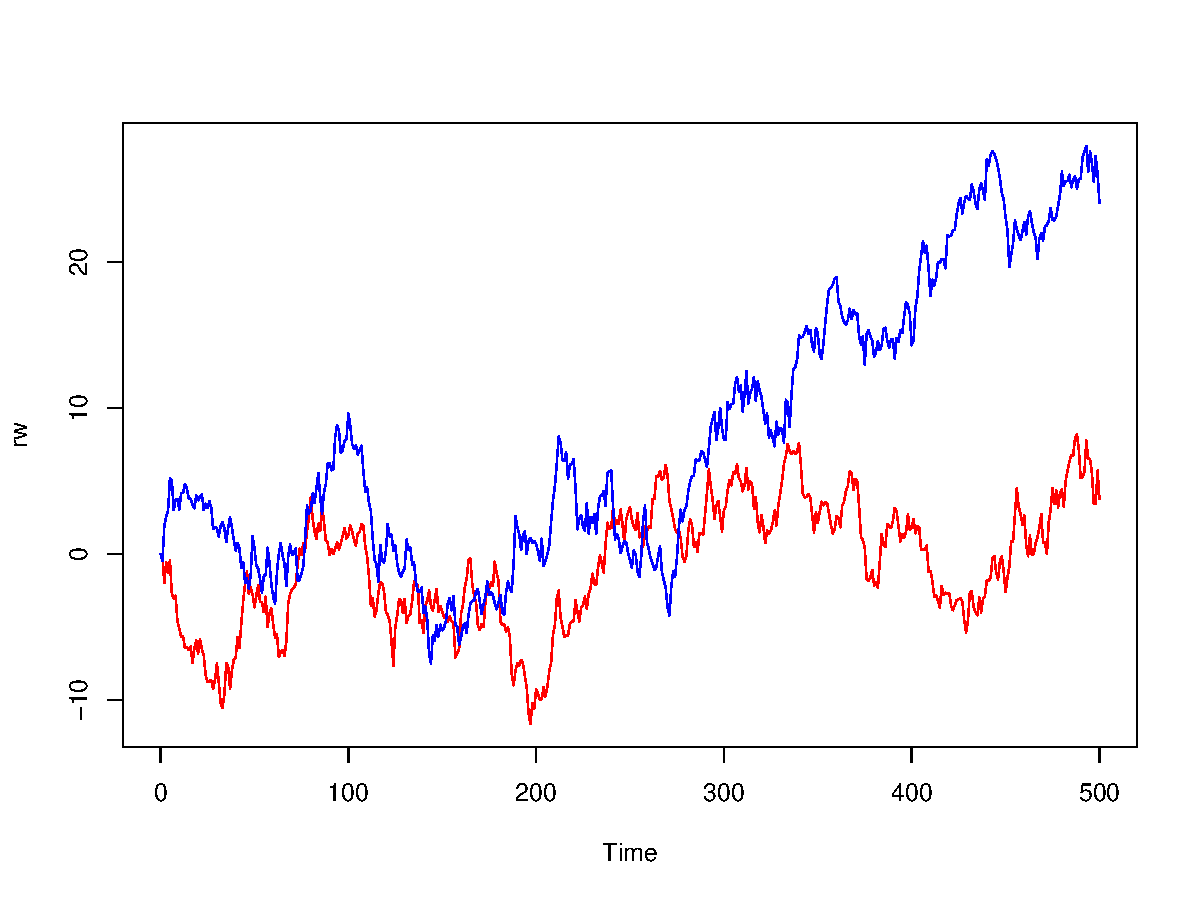
\includegraphics[scale=0.3]{graficos/espurio.pdf} 
		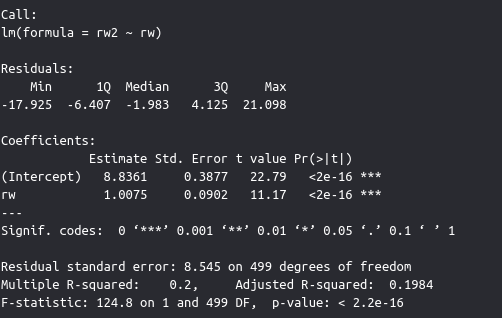
\includegraphics[scale=0.3]{graficos/reg.png} 
	\end{figure}
	Testes indicam que ambas as séries têm relação quando sabemos que isso não é verdade!
\end{frame}
\begin{frame}{Testando a presença de raiz unitária}
	\begin{wideitemize}
		\item Dadas as relações espúrias que são estimadas quando há tendência estocástica, é importante ser capaz de detectá-la nos dados.
		\begin{halfwideitemize}
			\item Também é importante diferenciar tendência estocástica de determinística, visto que a melhor transformação a se fazer em cada caso é diferente.
		\end{halfwideitemize}
		\item Considere o seguinte modelo para uma série de tempo $Y_t$:
		\begin{equation}
			\label{eq_rho}
			Y_t = \rho Y_{t-1} + \epsilon_t
		\end{equation}
		onde $\{\epsilon_t\}_t$ é ruído branco.
		\item Observe que:
		\begin{halfwideenumerate}
			\item Se $|\rho| < 1$, processo é I(0)
			\item Se $\rho = 1$, processo é I(1).
		\end{halfwideenumerate}
	\end{wideitemize}
\end{frame}
\begin{frame}{Teste de raiz unitária}
	\begin{halfwideitemize}
		\item Subtraindo $Y_{t-1}$ de ambos os lados de (14), obtemos:
		\begin{equation}
			\label{eq_no}
			\Delta Y_t = \gamma Y_{t-1} + \epsilon_t
		\end{equation}
		onde $\gamma = (\rho-1)$.
		\item Observe que:
		\begin{halfwideenumerate}
			\item Se $\gamma = 0$, processo é $I(1)$.
			\item Se $\gamma \in (-2, 0)$, processo é $I(0)$.
		\end{halfwideenumerate}
		\item Podemos usar um teste $t$ da nula de que $\gamma = 0$ contra a alternativa unicaudal $\gamma < 0$ como uma teste da nula de uma raiz unitária (contra a alternativa de que o processo é estacionário).
		\begin{halfwideitemize}
			\item Estatística de teste é $\hat{t} = \hat{\gamma}/\text{se}(\hat{\gamma})$, onde $\text{se}(\hat{\gamma})$ é o erro padrão homocedástico de Econometria I.
		\end{halfwideitemize}
		\item Como, sob a nula, o processo apresenta tendência estocástica, a distribuição de referência de $\hat{t}$ não é normal. \hyperlink{app_donsker}{\beamergotobutton{Detalhes}} \label{main_text}
		\begin{halfwideitemize}
			\item Valores críticos tabulados \citep{Dickey1979}.
		\end{halfwideitemize}
	\end{halfwideitemize}
\end{frame}

\begin{frame}{Teste de raiz unitária: modelo com intercepto}
	\begin{wideitemize}
		\item Às vezes, não temos certeza sobre os termos determinísticos de um processo.
		\item Nesse caso, é interessante considerar modelos como:
		\begin{equation}
			\label{eq_drift}
			\Delta Y_t = \alpha + \gamma Y_{t-1} + \epsilon_t
		\end{equation}
		\begin{halfwideitemize}
			\item Nesse modelo, se $\gamma = 0$, processo é um passeio aleatório com \textit{drift}; se $\gamma < 0$, é um AR(1) estacionário com intercepto.
			\item Estatística $t$ associada a $\gamma$ tem distribuição não normal sob $(\alpha, \gamma) = (0,0)$. Valores críticos tabulados \citep{Dickey1981}.
			\item Também é possível testar a nula de que $(\alpha,\gamma) =(0,0)$ usando um teste F. Nesse caso, a estatística também tem valores críticos não convencionais tabulados \citep{Dickey1981}.
		\end{halfwideitemize}
	\end{wideitemize}
\end{frame}

\begin{frame}{Teste de raiz unitária: modelo com intercepto e tendência linear}
	\begin{wideitemize}
		\item Podemos considerar, também:
		\begin{equation}
			\label{eq_trend}
			\Delta Y_t = \alpha + \beta \cdot t + \gamma Y_{t-1} + \epsilon_t
		\end{equation}
		\begin{halfwideitemize}
			\item Nesse modelo, se $\gamma = 0$, processo é um passeio aleatório com tendência quadrática; se $\gamma < 0$, é um AR(1) com tendência linear.
			\item Estatística $t$ associada a $\gamma$ tem distribuição não normal sob $(\beta, \gamma) = (0,0)$. Valores críticos tabulados \citep{Dickey1981}.
			\item Também é possível testar a nula de que $(\beta,\gamma) =(0,0)$ usando um teste F. Nesse caso, a estatística também tem valores críticos não convencionais tabulados \citep{Dickey1981}.
		\end{halfwideitemize}
	\end{wideitemize}
\end{frame}
\begin{frame}{Teste de raiz unitária: valores críticos da estatística $\hat{t}$}
	\begin{figure}
		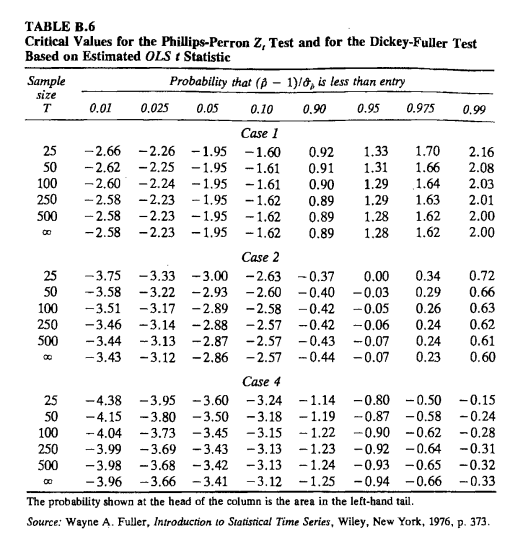
\includegraphics[scale=0.4]{graficos/valores_criticos_t.png}
	\end{figure}
\end{frame}

\begin{frame}{Teste de raiz unitária: valores críticos da estatística F}
	\begin{figure}
		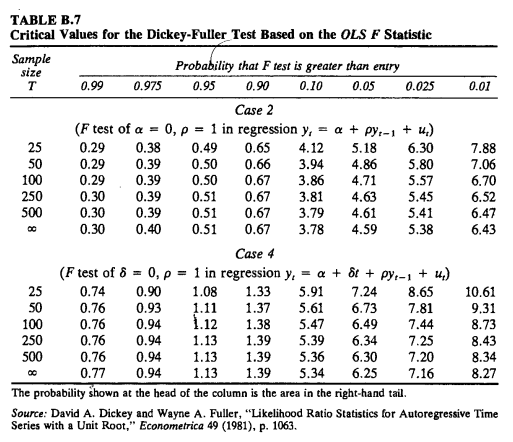
\includegraphics[scale=0.5]{graficos/valores_criticos_F.png}
	\end{figure}
\end{frame}

\begin{frame}{Teste Dickey-Fuller aumentado}
	\begin{halfwideitemize}
		\item A construção das estatísticas de teste nos modelos anteriores supõe que os erros $\{\epsilon_t\}$ comportem-se como ruídos brancos.
		\begin{halfwideitemize}
			\item Em particular, os erros não podem ser autocorrelacionados. 
		\end{halfwideitemize}
		\item \citet{Said1984} sugerem aumentar os modelos \eqref{eq_no}-\eqref{eq_trend} incluindo defasagens:
		\begin{equation}
			\label{eq_full}
			\begin{aligned}
				\Delta Y_t = \gamma Y_{t-1}  +\sum_{j=1}^k \kappa_j \Delta Y_{t-j} + u_t \\
				\Delta Y_t = \alpha + \gamma Y_{t-1}  +\sum_{j=1}^k \kappa_j \Delta Y_{t-j} + u_t
				\\
				\Delta Y_t = \alpha + \beta \cdot t + \gamma Y_{t-1} +  \sum_{j=1}^k\kappa_j \Delta Y_{t-j} + u_t
			\end{aligned}
		\end{equation}
		de modo que $\{u_t\}$ comporte-se \emph{aproximadamente} como ruído branco.
		\begin{itemize}
			\item Ideia é que, se número de defasagens $k$ varia como função lenta do tamanho amostral $T$, é possível capturar a correlação serial e ainda assim construir testes válidos com $T$ grande. 
		\end{itemize}
		
	\end{halfwideitemize}
\end{frame}

\begin{frame}{Selecionando defasagens}
		\begin{itemize}
			\item Nos modelos:
			\begin{equation}
				\tag{5}
		\begin{aligned}
			\Delta Y_t = \gamma Y_{t-1}  +\sum_{j=1}^k \kappa_j \Delta Y_{t-j} + u_t \\
			\Delta Y_t = \alpha + \gamma Y_{t-1}  +\sum_{j=1}^k \kappa_j \Delta Y_{t-j} + u_t
			\\
			\Delta Y_t = \alpha + \beta \cdot t + \gamma Y_{t-1} +  \sum_{j=1}^k\kappa_j \Delta Y_{t-j} + u_t
		\end{aligned}
	\end{equation}

			\item Teste de raiz unitária continua sendo de $H_0: \gamma = 0$ contra $H_1: \gamma < 0$.
			\begin{itemize}
				\vspace{-1em}
				\item Distribuição assintótica das estatísticas de teste, sob as nulas correspondentes, continua sendo a mesma.
			\end{itemize}
		\item \citet{Ng2001} propõem método MAIC para selecionar $k$.
		\begin{itemize}
			\item Ideia é encontrar $k$ tal que uma aproximação do erro quadrático médio de se prever $\Delta Y_t$ com base no modelo correspondente, \textbf{sob a nula} de raiz unitária, seja minimizada.
		\end{itemize}
	\end{itemize}
\end{frame}
\begin{frame}{Alternativa de \citet{Phillips1988}}
	\begin{itemize}
		\item \citet{Phillips1988} propõem uma alternativa ao teste ADF.
		\item Em vez de aumentar \eqref{eq_no}-\eqref{eq_trend} com defasagens, autores sugerem considerar os modelos \eqref{eq_no}-\eqref{eq_trend}, mas ajustar o erro padrão para torná-lo robusto a heterocedasticidade e correlação serial (mais adiante).
		\item Sob a nula $\gamma = 0$, distribuição assintótica dessa $\hat{t}$ coincide com a do teste ADF no modelo correspondente.
		\item Ao teste baseado nessa estatística damos o nome de Phillips-Perron (PP).
		\begin{itemize}
			\item Não focaremos nele nesse curso.
		\end{itemize} 
		
	\end{itemize}
\end{frame}
\begin{frame}{Procedimento sequencial para testar a presença de uma tendência estocástica}
	\begin{wideitemize}
		\item Da equação \eqref{eq_full} vimos três modelos diferentes em que podemos testar a presença de uma raiz unitária.
		\item A literatura sugere uma variedade de procedimentos {\color{blue}sequenciais} para testarmos se a série é I(1), começando do modelo mais geral ao mais simples.
		\item Nos próximos \textit{slides}, apresentamos uma versão desses procedimentos, baseada numa simplificação do procedimento descrito no Apêndice à Seção 4.4 de \citet{Enders2014}.
		
	\end{wideitemize}
\end{frame}

\begin{frame}{Procedimento Sequencial I}
	\begin{wideenumerate}
		\item Comece estimando o modelo mais geral:
		\begin{equation*}
			\begin{aligned}
				\Delta Y_t = \alpha + \beta \cdot t + \gamma Y_{t-1}  +\sum_{j=1}^k \kappa_j\Delta Y_{t-j} + u_t
			\end{aligned}
		\end{equation*}
		
		Teste $H_0: \gamma = 0$ contra a alternativa de que $H_1: \gamma < 0$ usando a estatística $\hat{t}$ e os valores críticos não normais para esse caso (\textit{slide} 10, caso 4).
		\begin{halfwideenumerate}
			\item Se rejeitamos a hipótese nula, concluímos que a série \textbf{não} apresenta raiz unitária.
			\item Se \textbf{não} rejeitamos a hipótese nula, fazemos o teste F da nula $(\beta, \gamma)=0$, usando os valores críticos do slide 11 (Caso 4).
			\begin{halfwideenumerate}
				\item Se \textbf{não} rejeitamos a hipótese  nula do teste $F$, concluímos que o modelo não apresenta tendência linear. Nesse caso, vamos à etapa 2 (próximo \textit{slide}).
				\item Se \textbf{rejeitamos} a hipótese nula do teste F, há evidências de tendência linear. Nesse caso, o teste $\hat{t}$ da nula $H_0: \gamma = 0$ contra a alternativa  $H_1: \gamma < 0$ pode ser feito usando a tabela da normal. Repita o teste com essa tabela. Se rejeitamos a nula, concluímos que a série \textbf{não} apresenta raiz unitária. Se não rejeitamos a nula, concluímos que a série \textbf{apresenta} raiz unitária.
			\end{halfwideenumerate}
		\end{halfwideenumerate}
		
	\end{wideenumerate}
	
\end{frame}

\begin{frame}{Procedimento Sequencial II}
	\begin{wideenumerate}
		\item[2] Se chegamos a essa etapa, não temos evidências de que haja uma tendência linear no modelo. Nesse caso, estimamos:
		\begin{equation*}
			\begin{aligned}
				\Delta Y_t = \alpha  + \gamma Y_{t-1}  +\sum_{j=1}^k \kappa_j \Delta Y_{t-j} + u_t
			\end{aligned}
		\end{equation*}
		
		Teste $H_0: \gamma = 0$ contra alternativa de que $H_1: \gamma < 0$ usando a estatística $\hat{t}$ e valores críticos não normais para esse caso (\textit{slide} 10, caso 2).
		\begin{halfwideenumerate}
			\item[2.1] Se rejeitamos a hipótese nula, concluímos que a série \textbf{não} apresenta raiz unitária.
			\item[2.2] Se \textbf{não} rejeitamos a hipótese nula, fazemos o teste F da nula $(\alpha, \gamma)=0$, usando os valores críticos do slide 11 (Caso 2).
			\begin{halfwideenumerate}
				\item[2.2.1] Se \textbf{não} rejeitamos a hipótese  nula do teste $F$, concluímos que o modelo não apresenta intercepto. Nesse caso, vamos à etapa 3 (próximo \textit{slide}).
				\item[2.2.2] Se \textbf{rejeitamos} a hipótese nula do teste F, há evidências de intercepto no modelo. Nesse caso, o teste $\hat{t}$ da nula $H_0: \gamma = 0$ contra a alternativa  $H_1: \gamma < 0$ pode ser feito usando a tabela da normal. Repita o teste com essa tabela. Se rejeitamos a nula, concluímos que a série \textbf{não} apresenta raiz unitária. Se não rejeitamos a nula, concluímos que a série \textbf{apresenta} raiz unitária.
			\end{halfwideenumerate}
		\end{halfwideenumerate}
		
	\end{wideenumerate}
	
\end{frame}

\begin{frame}{Procedimento Sequencial III}
	\begin{wideenumerate}
		\item[3] Se chegamos a essa etapa, não temos evidências de que haja uma tendência linear no modelo nem um intercepto. Nesse caso, estimamos:
		\begin{equation*}
			\begin{aligned}
				\Delta Y_t = \gamma Y_{t-1} +  \sum_{j=1}^k \kappa_j \Delta Y_{t-j} + u_t
			\end{aligned}
		\end{equation*}
		
		Teste a nula de $H_0: \gamma = 0$ contra a alternativa de que $H_1: \gamma < 0$ usando a estatística $\hat{t}$ e os valores críticos não normais para esse caso (\textit{slide} 10, caso 1). Se rejeitamos a hipótese nula, concluímos que a série \textbf{não} apresenta raiz unitária. Se não rejeitamos a nula, concluímos que a série \textbf{apresenta} raiz unitária.
		
	\end{wideenumerate}
	
\end{frame}

\begin{frame}{\citet{Elliott1996} }
	\begin{itemize}
		\item \citet{Elliott1996} estudam o poder dos testes de raiz unitária discutidos anteriormente.
		
	\end{itemize}
\end{frame}

\begin{frame}{Testando a presença de componentes determinísticos}
	\begin{halfwideitemize}
		\item A conclusão do procedimento sequencial anterior é uma afirmação: a série apresenta raiz unitária ou não.
		\item Se a série apresenta raiz unitária, vamos trabalhar como a série $Z_t = \Delta Y_t$.
		\item Se a série não apresenta unitária, trabalhamos com $Z_t = Y_t$.
		\item Podemos testar a presença de tendências determinísticas rodando:
		\begin{equation}
			Z_t = a + b \cdot t + \xi_t
		\end{equation}
		e testando a nula de que $b=0$ contra a alternativa de que $b \neq 0$ fazendo um teste $t$ com valores críticos normais.
		\begin{halfwideitemize}
			\item Se não rejeitamos a nula, trabalhamos com $Z_t$.
			\item Se rejeitamos a nula, o ideal é trabalhar com os resíduos do modelo, $\hat{\xi}_t$.
		\end{halfwideitemize}
	\end{halfwideitemize}
\end{frame}

\begin{frame}{Erros padrão HAC}
	\begin{halfwideitemize}
		\item Se rodamos o modelo (22) no \texttt{R} e usamos a função \texttt{summary} para fazer inferência, os erros padrão apresentados supõem homocedasticidade e não autocorrelação de $\xi_t$.
		\item Nesse caso, seria interessante computar erros padrão robustos a violações de ambas as hipóteses.
		\begin{halfwideitemize}
			\item A esse tipo de erro padrão damos o nome de HAC (\textit{heteroskedasticity and autocorrelation consistent}).
			\item Sua introdução na Economia se deve a \citet{Newey1987}.
		\end{halfwideitemize}
		\item Podemos usar esses erros padrão robustos via função \texttt{vcovHAC} do pacote \texttt{sandwich}.
	\end{halfwideitemize}
\end{frame}

\begin{frame}[allowframebreaks]{Referências}
	\printbibliography´
\end{frame}

\appendix
\begin{frame}{Derivação da distribuição assintótica de $\hat{\gamma}$ sob a nula $\gamma = 0$ }
	\label{app_donsker}
	
	\begin{itemize}
		\item Considere o estimador de MQO $\hat{\gamma}$ de \eqref{eq_no}.
		\item Note que
		$$\hat{\gamma} = \hat{\rho} - 1$$
		onde $\hat{\rho}$ é estimador de MQO de $\rho$ em \eqref{eq_rho}.
		\item Das propriedades de MQO, sabemos que:
		$$\hat{\gamma} -  \gamma = \frac{\sum_{t=2}^T y_{t-1}\epsilon_t}{\sum_{t=2}^T y_{t-1}^2}$$
		\item Defina a função com domínio $[0,1]$:
		
		$$X_T(r) = \begin{cases}
						\frac{\sum_{j=1}^{k}\epsilon_j}{T},& \text{se } k\leq r T <  (k+1)\, \\
						\frac{\sum_{j=1}^{T}\epsilon_j}{T}, & \text{se } r = 1
		\end{cases}$$

		\item Função em escada.
		\item \textbf{Sob a nula} $\gamma = 0$, $\sum_{j=1}^{k}\epsilon_j/T=  y_k/T$.
	\end{itemize}
\end{frame}

\begin{frame}{Gráfico de $r \mapsto X_T(r)$ sob a nula}
	\centering
	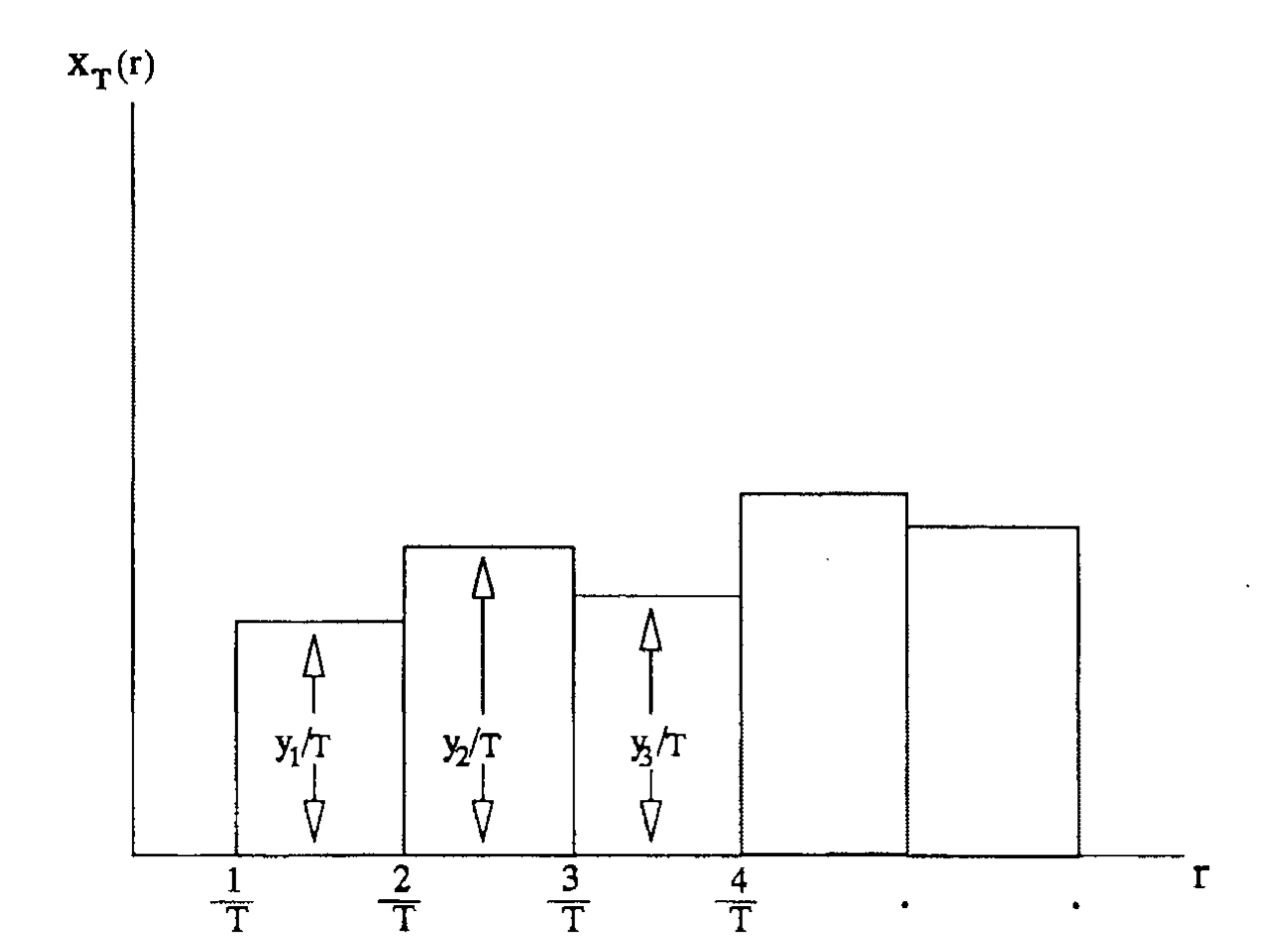
\includegraphics[scale=0.5]{graficos/escada.png}
\end{frame}

\begin{frame}{Teorema de Donsker}
	\begin{block}{Teorema de Donsker}
		Se os $\{\epsilon_j\}_{j}$ são iid com $\mathbb{E}[\epsilon_j]=0$ e $\sigma^2 < \infty$, então, quando $T \to \infty$
		
		$$\sqrt{T}X_T(\cdot) \Rightarrow \sigma B(\cdot)\, ,$$
		onde $B$ é um movimento Browniano (ou processo de Wiener) em $[0,1]$,
	\end{block}
	\begin{itemize}
		\item Teorema diz que a  função aleatória $\sqrt{T}X_T(\cdot)$ converge \emph{fracamente} para um Browniano.
		\begin{itemize}
			\item Convergência fraca: ``distribuição'' de $\sqrt{T}X_T(\cdot)$ converge para distribuição do Browniano.
		\end{itemize}
		\item Possível relaxar hipótese iid para ruído branco fracamente dependente \citep{Phillips1988}.
		\item Processo de Wiener é um processo estocástico (ou função aleatória) $t \mapsto B(t)$, cujas trajetórias são sempre contínuas, $B(0) = 0$, e onde os incrementos $B(t') - B(t)$ tem distribuição normal, com média zero e variância $(t'-t)$.
	\end{itemize}
\end{frame}

\begin{frame}{Processo de Wiener (cinco realizações)}
	\centering
	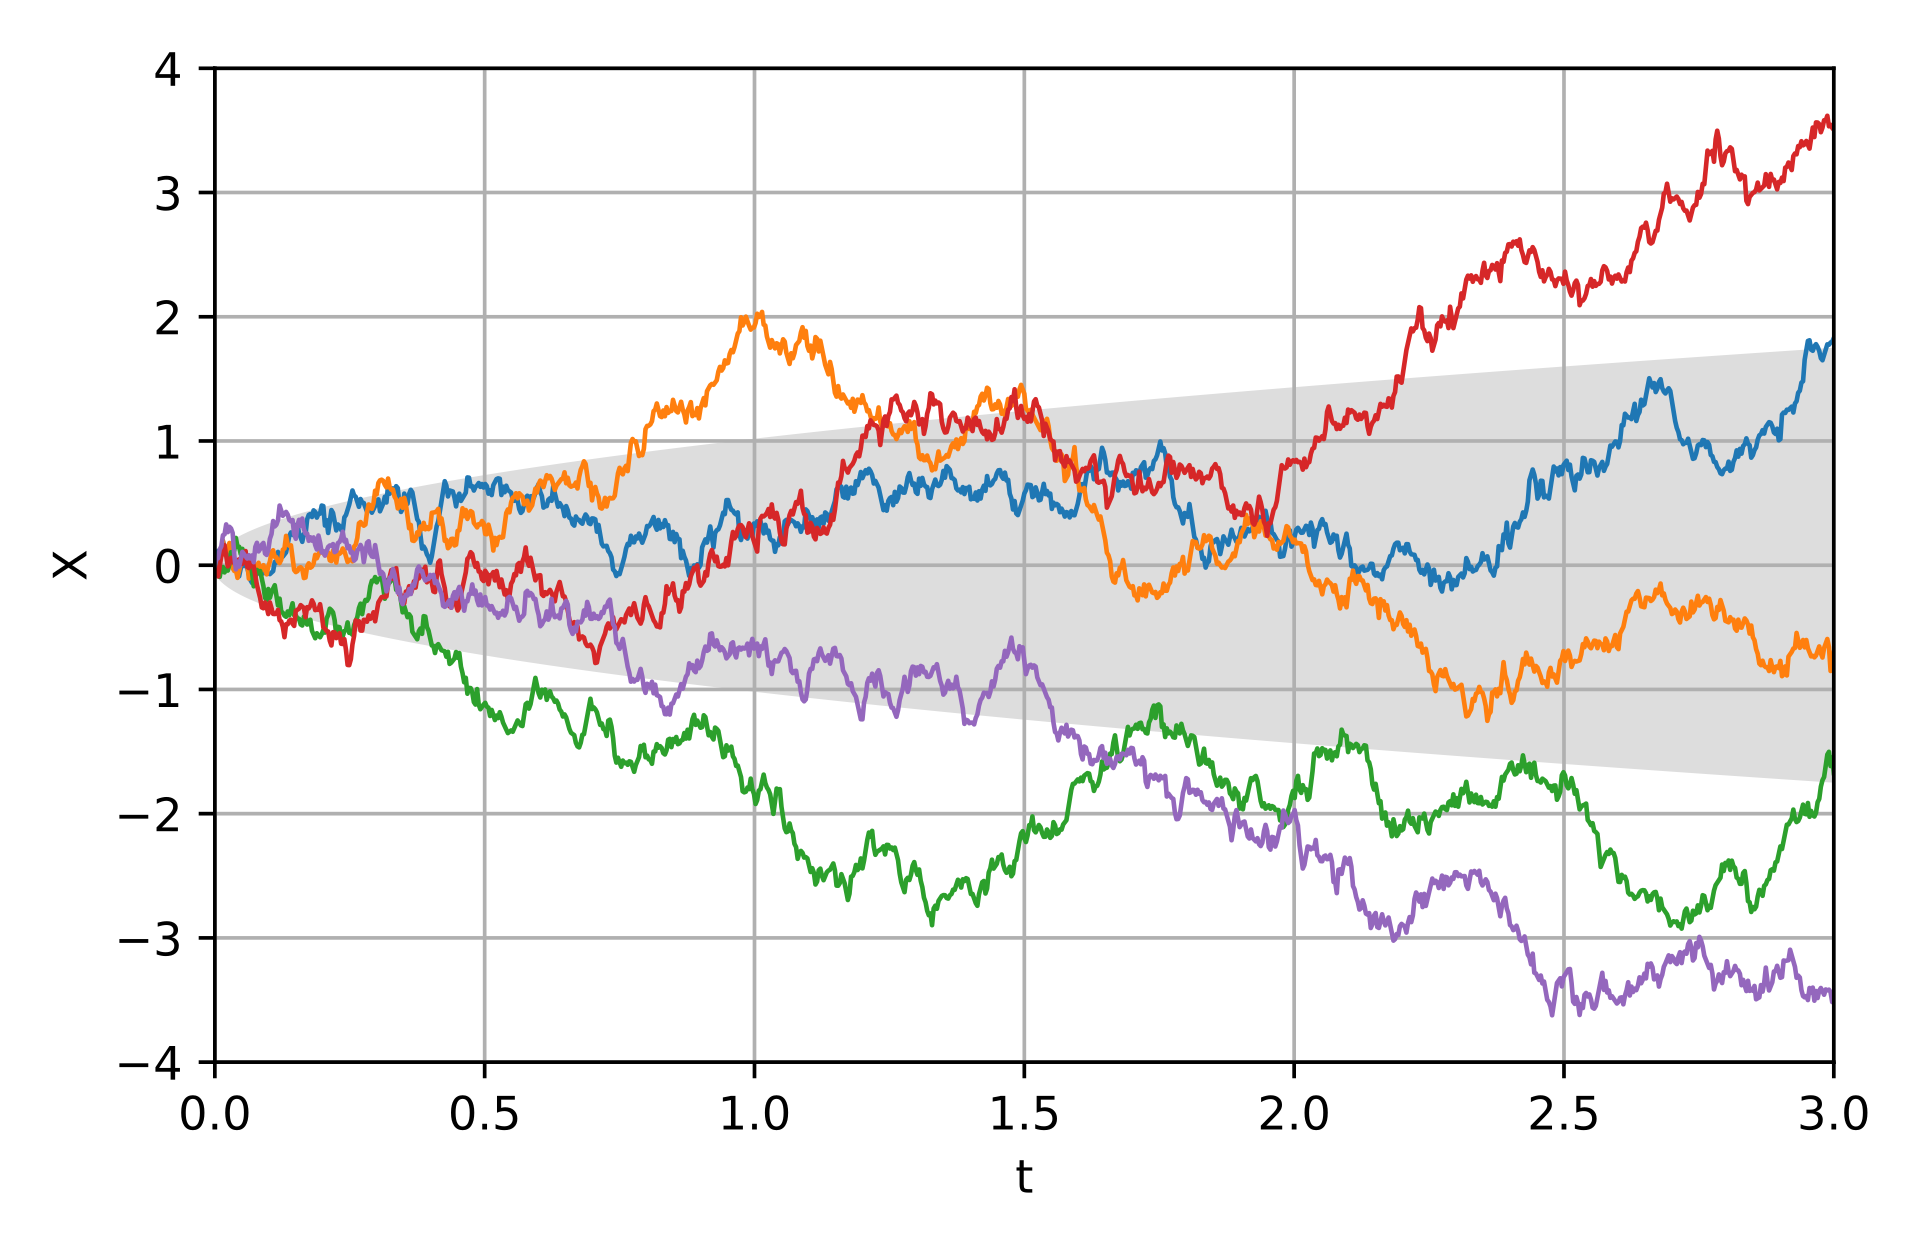
\includegraphics[scale=0.15]{graficos/wiener.png}
\end{frame}
\begin{frame}{Derivação da distribuição assintótica sob a nula}
	\begin{itemize}
		\item Note que, sob a nula:
		$$y_{t-1}^2 + 2y_{t-1}\epsilon_t+\epsilon_t^2 = (y_{t-1}+\epsilon_t)^2 = y_t^2$$
		\item Escrevendo em termos de $X_T(r)$, ficamos com:
		
		$$\hat{\gamma} -  \gamma = \frac{\sum_{t=2}^T y_{t-1}\epsilon_t}{\sum_{t=2}^Ty_{t-1}^2} =  \frac{1}{2} \frac{ T^2  X_T(1)^2 - y_{1}^2 - \sum_{t=2}^T \epsilon_t^2}{T^3 \int_0^1 X_T^2(u) du}\,,$$
		\item Pela LGN $\operatorname{plim}_{T \to \infty}\frac{1}{T-1}\sum_{t=2}^T \epsilon^2_t =\sigma^2$.
		\item Segue por preservação de convergência fraca em funções contínuas que:
		
		$$T(\hat{\gamma} -  \gamma) \Rightarrow \frac{B^2(1) -1}{2\int_0^1 B^2(u) du}$$
	\end{itemize}
	\hfill \hyperlink{main_text}{\beamerreturnbutton{Retornar à aula}} 
\end{frame}
\end{document}